% 若编译失败,且生成 .synctex(busy) 辅助文件,可能有两个原因:
% 1. 需要插入的图片不存在:Ctrl + F 搜索 'figure' 将这些代码注释/删除掉即可
% 2. 路径/文件名含中文或空格:更改路径/文件名即可

% ------------------------------------------------------------- %
% >> ------------------ 文章宏包及相关设置 ------------------ << %
% 设定文章类型与编码格式
\documentclass[UTF8]{report}		

% 本文特殊宏包
\usepackage{siunitx} % 埃米单位

% 本 .tex 专属的宏定义
    \def\V{\ \mathrm{V}}
    \def\mV{\ \mathrm{mV}}
    \def\kV{\ \mathrm{KV}}
    \def\KV{\ \mathrm{KV}}
    \def\MV{\ \mathrm{MV}}
    \def\A{\ \mathrm{A}}
    \def\mA{\ \mathrm{mA}}
    \def\kA{\ \mathrm{KA}}
    \def\KA{\ \mathrm{KA}}
    \def\MA{\ \mathrm{MA}}
    \def\O{\ \Omega}
    \def\mO{\ \Omega}
    \def\kO{\ \mathrm{K}\Omega}
    \def\KO{\ \mathrm{K}\Omega}
    \def\MO{\ \mathrm{M}\Omega}
    \def\Hz{\ \mathrm{Hz}}

% 自定义宏定义
    \def\N{\mathbb{N}}
    \def\F{\mathbb{F}}
    \def\Z{\mathbb{Z}}
    \def\Q{\mathbb{Q}}
    \def\R{\mathbb{R}}
    \def\C{\mathbb{C}}
    \def\T{\mathbb{T}}
    \def\S{\mathbb{S}}
    \def\A{\mathbb{A}}
    \def\I{\mathscr{I}}
    \def\Im{\mathrm{Im\,}}
    \def\Re{\mathrm{Re\,}}
    \def\d{\mathrm{d}}
    \def\p{\partial}

% 导入基本宏包
    \usepackage[UTF8]{ctex}     % 设置文档为中文语言
    \usepackage[colorlinks, linkcolor=blue, anchorcolor=blue, citecolor=blue, urlcolor=blue]{hyperref}  % 宏包:自动生成超链接 (此宏包与标题中的数学环境冲突)
    % \usepackage{hyperref}  % 宏包:自动生成超链接 (此宏包与标题中的数学环境冲突)
    % \hypersetup{
    %     colorlinks=true,    % false:边框链接 ; true:彩色链接
    %     citecolor={blue},    % 文献引用颜色
    %     linkcolor={blue},   % 目录 (我们在目录处单独设置),公式,图表,脚注等内部链接颜色
    %     urlcolor={orange},    % 网页 URL 链接颜色,包括 \href 中的 text
    %     % cyan 浅蓝色 
    %     % magenta 洋红色
    %     % yellow 黄色
    %     % black 黑色
    %     % white 白色
    %     % red 红色
    %     % green 绿色
    %     % blue 蓝色
    %     % gray 灰色
    %     % darkgray 深灰色
    %     % lightgray 浅灰色
    %     % brown 棕色
    %     % lime 石灰色
    %     % olive 橄榄色
    %     % orange 橙色
    %     % pink 粉红色
    %     % purple 紫色
    %     % teal 蓝绿色
    %     % violet 紫罗兰色
    % }

    % \usepackage{docmute}    % 宏包:子文件导入时自动去除导言区,用于主/子文件的写作方式,\include{./51单片机笔记}即可。注:启用此宏包会导致.tex文件capacity受限。
    \usepackage{amsmath}    % 宏包:数学公式
    \usepackage{mathrsfs}   % 宏包:提供更多数学符号
    \usepackage{amssymb}    % 宏包:提供更多数学符号
    \usepackage{pifont}     % 宏包:提供了特殊符号和字体
    \usepackage{extarrows}  % 宏包:更多箭头符号
    \usepackage{multicol}   % 宏包:支持多栏 
    \usepackage{graphicx}   % 宏包:插入图片
    \usepackage{float}      % 宏包:设置图片浮动位置
    %\usepackage{article}    % 宏包:使文本排版更加优美
    \usepackage{tikz}       % 宏包:绘图工具
    %\usepackage{pgfplots}   % 宏包:绘图工具
    \usepackage{enumerate}  % 宏包:列表环境设置
    \usepackage{enumitem}   % 宏包:列表环境设置

% 文章页面margin设置
    \usepackage[a4paper]{geometry}
        \geometry{top=1in}
        \geometry{bottom=1in}
        \geometry{left=0.75in}
        \geometry{right=0.75in}   % 设置上下左右页边距
        \geometry{marginparwidth=1.75cm}    % 设置边注距离(注释、标记等)

% 定义 solution 环境
\usepackage{amsthm}
\newtheorem{solution}{Solution}
        \geometry{bottom=1in}
        \geometry{left=0.75in}
        \geometry{right=0.75in}   % 设置上下左右页边距
        \geometry{marginparwidth=1.75cm}    % 设置边注距离(注释、标记等)

% 配置数学环境
    \usepackage{amsthm} % 宏包:数学环境配置
    % theorem-line 环境自定义
        \newtheoremstyle{MyLineTheoremStyle}% <name>
            {11pt}% <space above>
            {11pt}% <space below>
            {}% <body font> 使用默认正文字体
            {}% <indent amount>
            {\bfseries}% <theorem head font> 设置标题项为加粗
            {:}% <punctuation after theorem head>
            {.5em}% <space after theorem head>
            {\textbf{#1}\thmnumber{#2}\ \ (\,\textbf{#3}\,)}% 设置标题内容顺序
        \theoremstyle{MyLineTheoremStyle} % 应用自定义的定理样式
        \newtheorem{LineTheorem}{Theorem.\,}
    % theorem-block 环境自定义
        \newtheoremstyle{MyBlockTheoremStyle}% <name>
            {11pt}% <space above>
            {11pt}% <space below>
            {}% <body font> 使用默认正文字体
            {}% <indent amount>
            {\bfseries}% <theorem head font> 设置标题项为加粗
            {:\\ \indent}% <punctuation after theorem head>
            {.5em}% <space after theorem head>
            {\textbf{#1}\thmnumber{#2}\ \ (\,\textbf{#3}\,)}% 设置标题内容顺序
        \theoremstyle{MyBlockTheoremStyle} % 应用自定义的定理样式
        \newtheorem{BlockTheorem}[LineTheorem]{Theorem.\,} % 使用 LineTheorem 的计数器
    % definition 环境自定义
        \newtheoremstyle{MySubsubsectionStyle}% <name>
            {11pt}% <space above>
            {11pt}% <space below>
            {}% <body font> 使用默认正文字体
            {}% <indent amount>
            {\bfseries}% <theorem head font> 设置标题项为加粗
           % {:\\ \indent}% <punctuation after theorem head>
            {\\\indent}
            {0pt}% <space after theorem head>
            {\textbf{#3}}% 设置标题内容顺序
        \theoremstyle{MySubsubsectionStyle} % 应用自定义的定理样式
        \newtheorem{definition}{}

%宏包:有色文本框(proof环境)及其设置
    \usepackage[dvipsnames,svgnames]{xcolor}    %设置插入的文本框颜色
    \usepackage[strict]{changepage}     % 提供一个 adjustwidth 环境
    \usepackage{framed}     % 实现方框效果
        \definecolor{graybox_color}{rgb}{0.95,0.95,0.96} % 文本框颜色。修改此行中的 rgb 数值即可改变方框纹颜色,具体颜色的rgb数值可以在网站https://colordrop.io/ 中获得。(截止目前的尝试还没有成功过,感觉单位不一样)(找到喜欢的颜色,点击下方的小眼睛,找到rgb值,复制修改即可)
        \newenvironment{graybox}{%
        \def\FrameCommand{%
        \hspace{1pt}%
        {\color{gray}\small \vrule width 2pt}%
        {\color{graybox_color}\vrule width 4pt}%
        \colorbox{graybox_color}%
        }%
        \MakeFramed{\advance\hsize-\width\FrameRestore}%
        \noindent\hspace{-4.55pt}% disable indenting first paragraph
        \begin{adjustwidth}{}{7pt}%
        \vspace{2pt}\vspace{2pt}%
        }
        {%
        \vspace{2pt}\end{adjustwidth}\endMakeFramed%
        }



% 外源代码插入设置
    % matlab 代码插入设置
    \usepackage{matlab-prettifier}
        \lstset{style=Matlab-editor}    % 继承 matlab 代码高亮 , 此行不能删去
    \usepackage[most]{tcolorbox} % 引入tcolorbox包 
    \usepackage{listings} % 引入listings包
        \tcbuselibrary{listings, skins, breakable}
        \newfontfamily\codefont{Consolas} % 定义需要的 codefont 字体
        \lstdefinestyle{MatlabStyle_inc}{   % 插入代码的样式
            language=Matlab,
            basicstyle=\small\ttfamily\codefont,    % ttfamily 确保等宽 
            breakatwhitespace=false,
            breaklines=true,
            captionpos=b,
            keepspaces=true,
            numbers=left,
            numbersep=15pt,
            showspaces=false,
            showstringspaces=false,
            showtabs=false,
            tabsize=2,
            xleftmargin=15pt,   % 左边距
            %frame=single, % single 为包围式单线框
            frame=shadowbox,    % shadowbox 为带阴影包围式单线框效果
            %escapeinside=``,   % 允许在代码块中使用 LaTeX 命令 (此行无用)
            %frameround=tttt,    % tttt 表示四个角都是圆角
            framextopmargin=0pt,    % 边框上边距
            framexbottommargin=0pt, % 边框下边距
            framexleftmargin=5pt,   % 边框左边距
            framexrightmargin=5pt,  % 边框右边距
            rulesepcolor=\color{red!20!green!20!blue!20}, % 阴影框颜色设置
            %backgroundcolor=\color{blue!10}, % 背景颜色
        }
        \lstdefinestyle{MatlabStyle_src}{   % 插入代码的样式
            language=Matlab,
            basicstyle=\small\ttfamily\codefont,    % ttfamily 确保等宽 
            breakatwhitespace=false,
            breaklines=true,
            captionpos=b,
            keepspaces=true,
            numbers=left,
            numbersep=15pt,
            showspaces=false,
            showstringspaces=false,
            showtabs=false,
            tabsize=2,
        }
        \newtcblisting{matlablisting}{
            %arc=2pt,        % 圆角半径
            % 调整代码在 listing 中的位置以和引入文件时的格式相同
            top=0pt,
            bottom=0pt,
            left=-5pt,
            right=-5pt,
            listing only,   % 此句不能删去
            listing style=MatlabStyle_src,
            breakable,
            colback=white,   % 选一个合适的颜色
            colframe=black!0,   % 感叹号后跟不透明度 (为 0 时完全透明)
        }
        \lstset{
            style=MatlabStyle_inc,
        }



% table 支持
    \usepackage{booktabs}   % 宏包:三线表
    %\usepackage{tabularray} % 宏包:表格排版
    %\usepackage{longtable}  % 宏包:长表格
    %\usepackage[longtable]{multirow} % 宏包:multi 行列


% figure 设置
\usepackage{graphicx}   % 支持 jpg, png, eps, pdf 图片 
\usepackage{float}      % 支持 H 选项
\usepackage{svg}        % 支持 svg 图片
\usepackage{subcaption} % 支持子图
\svgsetup{
        % 指向 inkscape.exe 的路径
       inkscapeexe = C:/aa_MySame/inkscape/bin/inkscape.exe, 
        % 一定程度上修复导入后图片文字溢出几何图形的问题
       inkscapelatex = false                 
   }

% 图表进阶设置
    \usepackage{caption}    % 图注、表注
        \captionsetup[figure]{name=图}  
        \captionsetup[table]{name=表}
        \captionsetup{
            labelfont=bf, % 设置标签为粗体
            textfont=bf,  % 设置文本为粗体
            font=small  
        }
    \usepackage{float}     % 图表位置浮动设置 
        % \floatstyle{plaintop} % 设置表格标题在表格上方
        % \restylefloat{table}  % 应用设置


% 圆圈序号自定义
    \newcommand*\circled[1]{\tikz[baseline=(char.base)]{\node[shape=circle,draw,inner sep=0.8pt, line width = 0.03em] (char) {\small \bfseries #1};}}   % TikZ solution


% 列表设置
    \usepackage{enumitem}   % 宏包:列表环境设置
        \setlist[enumerate]{
            label=\bfseries(\arabic*) ,   % 设置序号样式为加粗的 (1) (2) (3)
            ref=\arabic*, % 如果需要引用列表项,这将决定引用格式(这里仍然使用数字)
            itemsep=0pt, parsep=0pt, topsep=0pt, partopsep=0pt, leftmargin=3.5em} 
        \setlist[itemize]{itemsep=0pt, parsep=0pt, topsep=0pt, partopsep=0pt, leftmargin=3.5em}
        \newlist{circledenum}{enumerate}{1} % 创建一个新的枚举环境  
        \setlist[circledenum,1]{  
            label=\protect\circled{\arabic*}, % 使用 \arabic* 来获取当前枚举计数器的值,并用 \circled 包装它  
            ref=\arabic*, % 如果需要引用列表项,这将决定引用格式(这里仍然使用数字)
            itemsep=0pt, parsep=0pt, topsep=0pt, partopsep=0pt, leftmargin=3.5em
        }  

% 文章默认字体设置
    \usepackage{fontspec}   % 宏包:字体设置
        \setmainfont{STKaiti}    % 设置中文字体为宋体字体
        \setCJKmainfont[AutoFakeBold=3]{STKaiti} % 设置加粗字体为 STKaiti 族,AutoFakeBold 可以调整字体粗细
        \setmainfont{Times New Roman} % 设置英文字体为Times New Roman


% 其它设置
    % 脚注设置
    \renewcommand\thefootnote{\ding{\numexpr171+\value{footnote}}}
    % 参考文献引用设置
        \bibliographystyle{unsrt}   % 设置参考文献引用格式为unsrt
        \newcommand{\upcite}[1]{\textsuperscript{\cite{#1}}}     % 自定义上角标式引用
    % 文章序言设置
        \newcommand{\cnabstractname}{序言}
        \newenvironment{cnabstract}{%
            \par\Large
            \noindent\mbox{}\hfill{\bfseries \cnabstractname}\hfill\mbox{}\par
            \vskip 2.5ex
            }{\par\vskip 2.5ex}


% 各级标题自定义设置
    \usepackage{titlesec}   
    % chapter
        \titleformat{\chapter}[hang]{\normalfont\Large\bfseries\centering}{题目}{10pt}{}
        \titlespacing*{\chapter}{0pt}{-30pt}{10pt} % 控制上方空白的大小
    % section
        \titleformat{\section}[hang]{\normalfont\large\bfseries}{\thesection}{8pt}{}
    % subsection
        %\titleformat{\subsubsection}[hang]{\normalfont\bfseries}{}{8pt}{}
    % subsubsection
        %\titleformat{\subsubsection}[hang]{\normalfont\bfseries}{}{8pt}{}

% 见到的一个有意思的对于公式中符号的彩色解释的环境
        \usepackage[dvipsnames]{xcolor}
        \usepackage{tikz}
        \usetikzlibrary{backgrounds}
        \usetikzlibrary{arrows,shapes}
        \usetikzlibrary{tikzmark}
        \usetikzlibrary{calc}
        
        \usepackage{amsmath}
        \usepackage{amsthm}
        \usepackage{amssymb}
        \usepackage{mathtools, nccmath}
        \usepackage{wrapfig}
        \usepackage{comment}
        
        % To generate dummy text
        \usepackage{blindtext}
        
        
        %color
        %\usepackage[dvipsnames]{xcolor}
        % \usepackage{xcolor}
        
        
        %\usepackage[pdftex]{graphicx}
        \usepackage{graphicx}
        % declare the path(s) for graphic files
        %\graphicspath{{../Figures/}}
        
        % extensions so you won't have to specify these with
        % every instance of \includegraphics
        % \DeclareGraphicsExtensions{.pdf,.jpeg,.png}
        
        % for custom commands
        \usepackage{xspace}
        
        % table alignment
        \usepackage{array}
        \usepackage{ragged2e}
        \newcolumntype{P}[1]{>{\RaggedRight\hspace{0pt}}p{#1}}
        \newcolumntype{X}[1]{>{\RaggedRight\hspace*{0pt}}p{#1}}
        
        % color box
        \usepackage{tcolorbox}
        
        
        % for tikz
        \usepackage{tikz}
        %\usetikzlibrary{trees}
        \usetikzlibrary{arrows,shapes,positioning,shadows,trees,mindmap}
        % \usepackage{forest}
        \usepackage[edges]{forest}
        \usetikzlibrary{arrows.meta}
        \colorlet{linecol}{black!75}
        \usepackage{xkcdcolors} % xkcd colors
        
        
        % for colorful equation
        \usepackage{tikz}
        \usetikzlibrary{backgrounds}
        \usetikzlibrary{arrows,shapes}
        \usetikzlibrary{tikzmark}
        \usetikzlibrary{calc}
        % Commands for Highlighting text -- non tikz method
        \newcommand{\highlight}[2]{\colorbox{#1!17}{$\displaystyle #2$}}
        %\newcommand{\highlight}[2]{\colorbox{#1!17}{$#2$}}
        \newcommand{\highlightdark}[2]{\colorbox{#1!47}{$\displaystyle #2$}}
        
        % my custom colors for shading
        \colorlet{mhpurple}{Plum!80}
        
        
        % Commands for Highlighting text -- non tikz method
        \renewcommand{\highlight}[2]{\colorbox{#1!17}{#2}}
        \renewcommand{\highlightdark}[2]{\colorbox{#1!47}{#2}}
        
        % Some math definitions
        \newcommand{\lap}{\mathrm{Lap}}
        \newcommand{\pr}{\mathrm{Pr}}
        
        \newcommand{\Tset}{\mathcal{T}}
        \newcommand{\Dset}{\mathcal{D}}
        \newcommand{\Rbound}{\widetilde{\mathcal{R}}}

% >> ------------------ 文章宏包及相关设置 ------------------ << %
% ------------------------------------------------------------- %



% ----------------------------------------------------------- %
% >> --------------------- 文章信息区 --------------------- << %
% 页眉页脚设置

\usepackage{fancyhdr}   %宏包:页眉页脚设置
    \pagestyle{fancy}
    \fancyhf{}
    \cfoot{\thepage}
    \renewcommand\headrulewidth{1pt}
    \renewcommand\footrulewidth{0pt}
    \rhead{数据结构与算法期末复习,\ 尹超,\ 2023K8009926003}
    \lhead{Homework}


%文档信息设置
\title{数据结构与算法期末复习\\ Homework}
\author{尹超\\ \footnotesize 中国科学院大学,北京 100049\\ Carter Yin \\ \footnotesize University of Chinese Academy of Sciences, Beijing 100049, China}
\date{\footnotesize 2024.8 -- 2025.1}
% >> --------------------- 文章信息区 --------------------- << %
% ----------------------------------------------------------- %     


% 开始编辑文章

\begin{document}
\zihao{5}           % 设置全文字号大小

% --------------------------------------------------------------- %
% >> --------------------- 封面序言与目录 --------------------- << %
% 封面
    \maketitle\newpage  
    \pagenumbering{Roman} % 页码为大写罗马数字
    \thispagestyle{fancy}   % 显示页码、页眉等

% 序言
    \begin{cnabstract}\normalsize 
        本文为笔者数据结构与算法的期末复习笔记。\par
        望老师批评指正。
    \end{cnabstract}
    \addcontentsline{toc}{chapter}{序言} % 手动添加为目录

% % 不换页目录
%     \setcounter{tocdepth}{0}
%     \noindent\rule{\textwidth}{0.1em}   % 分割线
%     \noindent\begin{minipage}{\textwidth}\centering 
%         \vspace{1cm}
%         \tableofcontents\thispagestyle{fancy}   % 显示页码、页眉等   
%     \end{minipage}  
%     \addcontentsline{toc}{chapter}{目录} % 手动添加为目录

% 目录
\setcounter{tocdepth}{4}                % 目录深度(为1时显示到section)
\tableofcontents                        % 目录页
\addcontentsline{toc}{chapter}{目录}    % 手动添加此页为目录
\thispagestyle{fancy}                   % 显示页码、页眉等 

% 收尾工作
    \newpage    
    \pagenumbering{arabic} 

% >> --------------------- 封面序言与目录 --------------------- << %
% --------------------------------------------------------------- %

\chapter{第五章 二叉树}

\section*{77}
\begin{graybox}
树是: \\
A. 有向连通图 \\
B. 无环平面图 \\
C. 连通无环图 \\
D. 有向无环图
\end{graybox}

\begin{solution}
正确答案是 C。

\textbf{详细分析:}

在图论中,树 (Tree) 通常指的是一个无向图,它满足以下等价条件之一:
\begin{enumerate}
    \item 是一个连通的无环图。
    \item 任意两个顶点之间存在唯一的一条简单路径。
    \item 是一个连通图,并且边的数量比顶点的数量少一 ($m = n-1$,其中 $m$ 是边数,$n$ 是顶点数)。
    \item 是一个无环图,并且边的数量比顶点的数量少一。
    \item 是一个无环图,并且添加任意一条新的边都会形成一个环。
    \item 是一个连通图,并且移除任意一条边都会使其不再连通(即每条边都是桥)。
\end{enumerate}

我们来分析各个选项:
\begin{itemize}
    \item \textbf{A. 有向连通图 (Directed connected graph):}
        树通常被定义为无向图。虽然有“有向树”(如根树、树形图)的概念,但题目中单独说“树”时,一般默认为无向树。此外,有向连通图可以包含环。例如,一个包含两个顶点和两条方向相反的边的有向图是连通的,但有环。

    \item \textbf{B. 无环平面图 (Acyclic planar graph):}
        树确实是无环的,并且所有树都是平面图(可以画在平面上而没有任何边相交)。然而,一个无环平面图不一定是连通的。例如,由两个不相交的树组成的图(即森林)是无环平面图,但它不是一棵树(因为它不连通)。

    \item \textbf{C. 连通无环图 (Connected acyclic graph):}
        这是树最标准和最直接的定义之一。一个图是树,当且仅当它是连通的并且不包含任何环。

    \item \textbf{D. 有向无环图 (Directed Acyclic Graph - DAG):}
        有向无环图是一个更广泛的概念。树(特指无向树)是无环的,但DAG是有向的。虽然有向树是DAG的一种特殊形式,但并非所有DAG都是树。例如,一个简单的有向路径 $A \rightarrow B \rightarrow C$ 是一个DAG,但如果考虑其底层的无向图,它是一棵树。然而,一个更复杂的DAG,比如 $A \rightarrow B, A \rightarrow C, B \rightarrow D, C \rightarrow D$,其底层的无向图可能包含环(如果 $A,B,C,D$ 形成一个菱形结构,但边是有向的以避免有向环)。更重要的是,DAG不要求连通性(在有向图的连通性定义下,如强连通或弱连通)。
\end{itemize}

因此,最准确描述树的选项是“连通无环图”。
\end{solution}


\section*{78}
\begin{graybox}
在一棵树中,顶点p是顶点v的父亲,则它
们的高度的关系是: \\
A. height(v) < height(p) \\
B. height(v) = height(p) - 1 \\
C. height(v) = height(p) + 1 \\
D. height(p) < height(v)
\end{graybox}

\begin{solution}
正确答案是 A。

\textbf{详细分析:}

首先,我们明确树中节点高度的定义:
\textbf{节点的高度 (Height of a node)}:从该节点到其子树中某个叶子节点的最长路径的长度(边的数量)。叶子节点的高度为0。

设 $H(x)$ 表示节点 $x$ 的高度。
题目中给出顶点 $p$ 是顶点 $v$ 的父亲。

考虑节点 $p$ 的高度 $H(p)$。根据定义,$H(p)$ 是从 $p$ 出发到其子树中某个叶子节点的最长路径的长度。
这条最长路径必然会经过 $p$ 的一个孩子节点。设 $c_1, c_2, \ldots, c_k$ 是 $p$ 的所有孩子节点。
则 $p$ 的高度可以通过其孩子节点的高度递归定义:
$H(p) = 1 + \max \{ H(c_1), H(c_2), \ldots, H(c_k) \}$

由于 $v$ 是 $p$ 的一个孩子节点,所以 $v$ 是 $\{c_1, c_2, \ldots, c_k\}$ 中的一个。
因此,$H(v) \le \max \{ H(c_1), H(c_2), \ldots, H(c_k) \}$。

将此代入 $H(p)$ 的表达式中:
$H(p) = 1 + \max \{ H(c_i) \}$
$H(p) \ge 1 + H(v)$


从不等式 $H(p) \ge 1 + H(v)$,我们可以推导出:
$H(p) - 1 \ge H(v)$
或者写成 $H(v) \le H(p) - 1$。

因为高度是路径长度,是非负整数。
如果 $H(v) \le H(p) - 1$,那么必然有 $H(v) < H(p)$。
(证明:假设 $H(v) \ge H(p)$。如果 $H(v) = H(p)$,则 $H(p) \le H(p) - 1 \Rightarrow 0 \le -1$,矛盾。如果 $H(v) > H(p)$,则 $H(v) \le H(p) - 1$ 更不可能成立。所以必须 $H(v) < H(p)$。)

现在我们分析选项:
\begin{itemize}
    \item \textbf{A. height(v) < height(p)}: 根据上面的推导 $H(v) \le H(p) - 1$,这个关系总是成立的。
    \item \textbf{B. height(v) = height(p) - 1}: 这个关系仅在 $v$ 恰好是构成从 $p$ 出发的最长路径的那个孩子节点(或者之一)时成立。也就是说,当 $H(v) = \max \{ H(c_i) \}$ 时, $H(p) = 1 + H(v)$,即 $H(v) = H(p) - 1$。但如果 $p$ 有另一个孩子 $v'$ 使得 $H(v') > H(v)$,那么 $H(p) = 1 + H(v')$,此时 $H(v) < H(p) - 1$。所以这个关系不总是成立。
    \item \textbf{C. height(v) = height(p) + 1}: 这意味着 $H(p) = H(v) - 1$,即 $H(p) < H(v)$,这与我们的推导 $H(p) > H(v)$ 相矛盾。所以这是错误的。
    \item \textbf{D. height(p) < height(v)}: 这与我们的推导 $H(p) > H(v)$ 相矛盾。所以这是错误的。
\end{itemize}

由于关系 A ($H(v) < H(p)$) 是从 $H(v) \le H(p) - 1$ 直接得出的,并且对于任何父子关系都成立,而关系 B 只是一个特例,因此 A 是描述它们高度之间普遍关系的正确选项。

\textbf{举例说明:}
\begin{enumerate}
    \item 树: p $\rightarrow$ v (v是叶子)
        $H(v) = 0$
        $H(p) = 1 + H(v) = 1 + 0 = 1$
        $H(v) < H(p)$ (0 < 1) - 成立。
        $H(v) = H(p) - 1$ (0 = 1 - 1) - 成立。

    \item 树:
        \begin{center}
        p \\
        / \textbackslash \\
        v   w \\
        (叶子) (叶子)
        \end{center}
        $H(v) = 0$
        $H(w) = 0$
        $H(p) = 1 + \max(H(v), H(w)) = 1 + \max(0, 0) = 1$.
        对于孩子 $v$: $H(v) < H(p)$ (0 < 1) - 成立。 $H(v) = H(p) - 1$ (0 = 1 - 1) - 成立。

    \item 树:
        \begin{center}
        p \\
        / \textbackslash \\
        v   w \\
        (叶子) | \\
              x (叶子)
        \end{center}
        $H(v) = 0$
        $H(x) = 0$
        $H(w) = 1 + H(x) = 1$
        $H(p) = 1 + \max(H(v), H(w)) = 1 + \max(0, 1) = 1 + 1 = 2$.
        对于孩子 $v$:
        $H(v) = 0, H(p) = 2$.
        $H(v) < H(p)$ (0 < 2) - 成立。
        $H(v) = H(p) - 1$ (0 = 2 - 1 = 1) - 不成立。
        对于孩子 $w$:
        $H(w) = 1, H(p) = 2$.
        $H(w) < H(p)$ (1 < 2) - 成立。
        $H(w) = H(p) - 1$ (1 = 2 - 1 = 1) - 成立。
\end{enumerate}
从例子中可以看出,A 选项始终成立,而 B 选项不一定成立。因此,A 是它们高度之间更普遍的关系。
\end{solution}

\section*{79}
\begin{graybox}
用父节点+孩子节点的方法存储n个节点的树,
需要的空间是: \\
A. O(1) \\
B. O(n) \\
C. O(nlogn) \\
D. O($n^2$)
\end{graybox}

\begin{solution}
正确答案是 B。

\textbf{详细分析:}

“用父节点+孩子节点的方法存储n个节点的树”通常指的是每个节点存储以下信息:
\begin{enumerate}
    \item 节点自身的数据。
    \item 指向其父节点的指针(根节点的父指针可能为null)。
    \item 指向其所有孩子节点的信息(例如,一个孩子节点的列表或链表,或者使用“长子-兄弟”表示法)。
\end{enumerate}

我们来分析所需空间:
\begin{itemize}
    \item \textbf{节点数据:} 存储 $n$ 个节点的数据,每个节点的数据占用固定空间(或平均固定空间),总空间为 $O(n)$。
    \item \textbf{父节点指针:} 每个节点(除了可能的根节点,但为了统一分析,可以认为每个节点都有一个父指针的空间分配)存储一个指向其父节点的指针。对于 $n$ 个节点,这需要 $n$ 个指针,空间复杂度为 $O(n)$。
    \item \textbf{孩子节点信息:}
        \begin{itemize}
            \item \textbf{孩子链表/列表表示:} 每个节点维护一个列表(如链表或动态数组)来存储指向其直接孩子节点的指针。在一棵有 $n$ 个节点的树中,总共有 $n-1$ 条边,每条边代表一个父子关系。因此,所有孩子列表中指针的总数是 $n-1$。存储这些指针需要 $O(n)$ 的空间。列表结构本身可能还有一些额外的开销(例如链表中的next指针),但这些开销通常也与孩子数量成正比,总体上仍是 $O(n)$。
            \item \textbf{长子-兄弟表示法 (First-child, Next-sibling):} 每个节点存储两个指针:一个指向其第一个孩子(长子),另一个指向其下一个兄弟。如果也存储父指针,则每个节点固定存储3个指针。对于 $n$ 个节点,总共需要 $3n$ 个指针,空间复杂度为 $O(n)$。这种方法也能有效地表示父子关系。
        \end{itemize}
\end{itemize}

综合来看,无论是哪种具体的“孩子节点”存储方式(只要是合理高效的),存储 $n$ 个节点的数据、父节点指针以及孩子节点信息所需的总空间都与节点数量 $n$ 成线性关系。

因此,总的空间复杂度为 $O(n) + O(n) + O(n) = O(n)$。

分析选项:
\begin{itemize}
    \item \textbf{A. O(1):} 存储 $n$ 个节点不可能只用常数空间。
    \item \textbf{B. O(n):} 符合上述分析。
    \item \textbf{C. O(nlogn):} 通常不适用于这种基本的树存储方法。
    \item \textbf{D. O($n^2$):} 除非使用非常低效的表示方法(如为每个节点预留 $n$ 个孩子指针的空间,无论实际孩子数量多少,或者使用邻接矩阵),否则对于树的这种描述,空间复杂度不会是 $O(n^2)$。
\end{itemize}

所以,最合理的答案是 $O(n)$。
\end{solution}


\section*{80}
\begin{graybox}
一棵高度为h,节点数为n的真二叉树的特
点是: \\
A. h = O(log$_2$n) \\
B. 真的是二叉树,而不会是其他种类的树 \\
C. 不存在只有一个父亲的节点 \\
D. 不存在只有一个孩子的节点
\end{graybox}

\begin{solution}
正确答案是 D。

\textbf{详细分析:}

“真二叉树”(Proper Binary Tree 或 Strictly Binary Tree)通常指的是这样一种二叉树:树中的每个节点要么是叶子节点(没有孩子),要么正好有两个孩子。不允许节点只有一个孩子。

我们来分析各个选项:
\begin{itemize}
    \item \textbf{A. h = O(log$_2$n)}:
        这个关系描述的是平衡二叉树的高度。一棵真二叉树不一定是平衡的。例如,一个“倾斜”的真二叉树(其中每个内部节点都有两个孩子,但树向一侧延伸得很长)的高度 $h$ 可以是 $O(n)$。例如,考虑一个链状结构,其中每个节点都有一个孩子是内部节点,另一个孩子是叶子节点。若有 $k$ 个这样的内部节点,则总节点数 $n = 2k+1$,高度 $h=k=(n-1)/2$。因此,A 选项不总是成立。

    \item \textbf{B. 真的是二叉树,而不会是其他种类的树}:
        这是一个定义性的陈述,说明真二叉树是二叉树的一个特例。它并没有指出真二叉树区别于其他一般二叉树的结构特点。

    \item \textbf{C. 不存在只有一个父亲的节点}:
        在任何树结构中(除了根节点),每个非根节点都有且仅有一个父亲节点。根节点没有父亲节点。这个选项的表述容易引起混淆,并且不能准确描述真二叉树的特性。

    \item \textbf{D. 不存在只有一个孩子的节点}:
        这正是真二叉树(Proper/Strict Binary Tree)的定义。在真二叉树中,每个节点的度(孩子数量)要么是0(叶子节点),要么是2(内部节点)。不存在度为1的节点。
\end{itemize}

因此,最能准确描述真二叉树特点的是选项 D。
\end{solution}


\section*{81}
\begin{graybox}
在长子-兄弟表示法中,树中某节点的长子相当
于二叉树中的: \\
A. 幼子 \\
B. 左子 \\
C. 右子 \\
D. 长子
\end{graybox}

\begin{solution}
正确答案是 B。

\textbf{详细分析:}

长子-兄弟表示法(First-child, Next-sibling representation)是一种将任意树(多叉树)转换为二叉树(或者说,用二叉树的结构来存储多叉树)的常用方法。

在这种表示法中,对于原树中的任意一个节点 N:
\begin{itemize}
    \item N 的第一个孩子(长子)在转换后的二叉树中成为 N 的 \textbf{左孩子}。
    \item N 的下一个兄弟节点(即与 N 有相同父节点,并且在父节点的孩子序列中紧跟在 N 之后的节点)在转换后的二叉树中成为 N 的 \textbf{右孩子}。
\end{itemize}

因此,树中某节点的“长子”(第一个孩子)在长子-兄弟表示法所对应的二叉树中,相当于该节点的“左子”。

\textbf{举例:}
假设有如下多叉树:
\begin{verbatim}
      A
     /|\
    B C D
   /|   |
  E F   G
\end{verbatim}

使用长子-兄弟表示法转换成的二叉树结构如下:
\begin{itemize}
    \item A 的长子是 B $\rightarrow$ B 是 A 的左孩子。
    \item B 的下一个兄弟是 C $\rightarrow$ C 是 B 的右孩子。
    \item C 的下一个兄弟是 D $\rightarrow$ D 是 C 的右孩子。
    \item D 没有下一个兄弟 $\rightarrow$ D 的右孩子为空。
    \item B 的长子是 E $\rightarrow$ E 是 B 的左孩子。
    \item E 的下一个兄弟是 F $\rightarrow$ F 是 E 的右孩子。
    \item F 没有下一个兄弟 $\rightarrow$ F 的右孩子为空。
    \item C 没有孩子 $\rightarrow$ C 的左孩子为空。
    \item D 的长子是 G $\rightarrow$ G 是 D 的左孩子。
    \item G 没有孩子,也没有兄弟 $\rightarrow$ G 的左右孩子都为空。
\end{itemize}

转换后的二叉树大致形态:
\begin{verbatim}
      A
     /
    B
   / \
  E   C
   \   \
    F   D
       /
      G
\end{verbatim}

从这个例子可以看出,原树中节点 A 的长子 B,在二叉树中是 A 的左子。原树中节点 B 的长子 E,在二叉树中是 B 的左子。

所以,选项 B "左子" 是正确的。
\end{solution}



\section*{82}
\begin{graybox}
设二叉树有n个节点,高度为h.在其中插
入一个新的节点,高度发生改变的节点个数为: \\
A. O(1) \\
B. O(n) \\
C. O(h) \\
D. O(hlog$_{2}$(n))
\end{graybox}

\begin{solution}
正确答案是 C。

\textbf{详细分析:}

首先,我们回顾节点高度的定义:
\textbf{节点的高度 (Height of a node)}:从该节点到其子树中某个叶子节点的最长路径的长度(边的数量)。叶子节点的高度为0。
树的高度是其根节点的高度。

当在一个二叉树中插入一个新的节点时,这个新节点通常是作为某个现有节点的子节点(如果该现有节点有空余的子节点位置)或者替换一个叶子节点(如果插入操作涉及将叶子节点变为内部节点并添加新叶子)。在最简单的情况下,新节点被添加为一个新的叶子节点。

\begin{enumerate}
    \item \textbf{新插入节点的高度:} 新插入的节点自身将成为一个叶子节点(或者其子树只包含它自己),因此其高度为0。

    \item \textbf{哪些节点的度可能改变?}
        只有新插入节点的父节点以及其所有祖先节点的度才有可能发生改变。

    \item \textbf{哪些节点的高度可能改变?}
        \begin{itemize}
            \item 新插入节点的父节点 $P$:如果新节点的插入使得从 $P$ 到其子树中叶子节点的最长路径长度发生变化,则 $P$ 的高度会改变。例如,如果 $P$ 原本是叶子节点(高度为0),插入新节点后 $P$ 的高度变为1。或者,如果 $P$ 原本有一个孩子,新插入的节点是 $P$ 的另一个孩子,并且这条新路径($P \rightarrow$ 新节点)比原来从 $P$ 出发的最长路径更长或一样长(但之前是另一条路径决定的高度),则 $P$ 的高度可能改变。
            \item $P$ 的父节点(即新节点的祖父节点)以及更高层的祖先节点:如果一个节点 $A$ 的高度发生改变,那么 $A$ 的父节点的高度也可能随之改变,这个影响可能一直向上传播到根节点。
        \end{itemize}

    \item \textbf{改变高度的节点数量:}
        发生高度改变的节点必然是新插入节点的祖先节点(包括其父节点)。
        在一个高度为 $h$ 的树中,从任何一个叶子节点到根节点的路径上最多有 $h+1$ 个节点(包括叶子和根)。因此,新插入的节点最多有 $h$ 个祖先节点(不包括新节点自身)。
        在最坏的情况下,从新插入节点的父节点一直到根节点,所有这些祖先节点的高度都可能发生改变。这种情况通常发生在插入操作增加了树的整体高度时,或者插入点位于原先决定各祖先高度的关键路径上。
        因此,高度发生改变的节点个数最多为 $h$(即新插入节点的父节点及其所有祖先,直到根节点)。

    \item \textbf{复杂度分析:}
        由于最多有 $h$ 个祖先节点的高度可能改变,所以发生高度改变的节点个数为 $O(h)$。
\end{enumerate}

分析选项:
\begin{itemize}
    \item \textbf{A. O(1):} 这是可能的,例如,如果插入一个新节点,其父节点 $P$ 的高度没有改变(因为 $P$ 的另一子树远比新插入的节点形成的路径要高),那么 $P$ 的祖先节点的高度也不会改变。但这只是最好情况。
    \item \textbf{B. O(n):} 不太可能。只有新插入节点的祖先才可能改变高度。
    \item \textbf{C. O(h):} 这是最坏情况下的上界。
    \item \textbf{D. O(hlog$_{2}$(n))}: 这个表达式没有直接的依据。$h$ 本身就是路径长度的度量。
\end{itemize}

因此,在最坏情况下,从新插入节点的父节点到根节点的所有 $h$ 个节点的高度都可能改变。所以,高度发生改变的节点个数为 $O(h)$。
\end{solution}

\section*{83}
\begin{graybox}
对以下二叉树进行先序遍历:
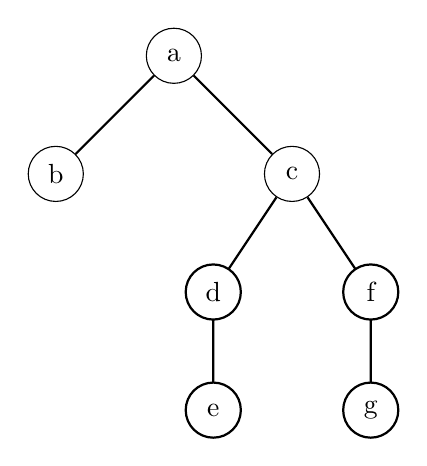
\begin{tikzpicture}[
    % 节点样式定义
    node style/.style={
        circle,              % 圆形节点
        draw,                % 绘制边框
        fill=white,          % 填充白色
        minimum size=0.7cm,  % 最小尺寸
        inner sep=0pt        % 内部填充为0
    },
    % 箭头样式定义 (模仿图中较粗的带箭头的斜线)
    thick arrow style/.style={
        draw=gray,           % 灰色绘制
        line width=3pt,      % 较粗的线宽
        -{Latex[length=4mm, width=4mm]} % 大箭头,这里使用Latex[]来调整大小
    },
    % 边样式定义
    edge from parent/.style={
        draw,                % 绘制
        thick,               % 粗线
        -                % 没有箭头
    },
    % 节点间距
    level 1/.style={sibling distance=3cm}, % 第一层子节点间距
    level 2/.style={sibling distance=2cm}, % 第二层子节点间距
    level 3/.style={sibling distance=1.5cm} % 第三层子节点间距
]

% 定义节点
\node[node style] (a) {a}
    child { node[node style] (b) {b} }
    child { node[node style] (c) {c}
        child { node[node style] (d) {d}
            child { node[node style] (e) {e} }
        }
        child { node[node style] (f) {f}
            child { node[node style] (g) {g} }
        }
    };

\end{tikzpicture}
刚访问完节点d时(迭代实现2)栈中的元素从栈顶到栈底依次为: \\
A. e \\
B. g,f \\
C. f,g \\
D. f
\end{graybox}

\begin{solution}
正确答案是 D。

\textbf{详细分析:}
我们使用标准的迭代先序遍历算法,该算法使用一个栈。算法步骤如下:
\begin{enumerate}
    \item 初始化一个空栈 S。
    \item 将根节点压入栈 S。
    \item 当栈 S 不为空时:
    \begin{enumerate}
        \item 从栈 S 中弹出一个节点,设为 \texttt{curr}。
        \item 访问节点 \texttt{curr}。
        \item 如果 \texttt{curr} 的右孩子存在,则将其右孩子压入栈 S。
        \item 如果 \texttt{curr} 的左孩子存在,则将其左孩子压入栈 S。(注意顺序:先压右孩子,再压左孩子,这样弹出时左孩子先被处理)。
    \end{enumerate}
\end{enumerate}

树的结构为:
\begin{verbatim}
      a
     / \
    b   c
       / \
      d   f
     /   /
    e   g
\end{verbatim}
栈的表示中,列表的右侧为栈顶。

\textbf{遍历过程追踪:}
\begin{enumerate}
    \item 初始:S = \texttt{[]}, 已访问 = \texttt{[]}
    \item \texttt{S.push(a)} $\rightarrow$ S = \texttt{[a]}
    \item 弹出 \texttt{a}, 访问 \texttt{a}. 已访问 = \texttt{[a]}.
          \texttt{S.push(c)} (a的右孩子) $\rightarrow$ S = \texttt{[c]}
          \texttt{S.push(b)} (a的左孩子) $\rightarrow$ S = \texttt{[c, b]}
    \item 弹出 \texttt{b}, 访问 \texttt{b}. 已访问 = \texttt{[a, b]}.
          b没有右孩子.
          b没有左孩子.
          S = \texttt{[c]}
    \item 弹出 \texttt{c}, 访问 \texttt{c}. 已访问 = \texttt{[a, b, c]}.
          \texttt{S.push(f)} (c的右孩子) $\rightarrow$ S = \texttt{[f]}
          \texttt{S.push(d)} (c的左孩子) $\rightarrow$ S = \texttt{[f, d]}
    \item 弹出 \texttt{d}, 访问 \texttt{d}. 已访问 = \texttt{[a, b, c, d]}.
          \textbf{此时是“刚访问完节点d时”。}
          栈 S 的内容为 \texttt{[f]}。
          从栈顶到栈底的元素依次为: \texttt{f}。
    \item (继续 \texttt{d} 的处理)
          \texttt{d} 没有右孩子.
          \texttt{S.push(e)} (d的左孩子) $\rightarrow$ S = \texttt{[f, e]}
    \item 弹出 \texttt{e}, 访问 \texttt{e}. 已访问 = \texttt{[a, b, c, d, e]}.
          S = \texttt{[f]}
    \item 弹出 \texttt{f}, 访问 \texttt{f}. 已访问 = \texttt{[a, b, c, d, e, f]}.
          \texttt{f} 没有右孩子.
          \texttt{S.push(g)} (f的左孩子) $\rightarrow$ S = \texttt{[g]}
    \item 弹出 \texttt{g}, 访问 \texttt{g}. 已访问 = \texttt{[a, b, c, d, e, f, g]}.
          S = \texttt{[]}
\end{enumerate}
根据追踪,在刚访问完节点 \texttt{d} 时,栈中的元素从栈顶到栈底依次为 \texttt{f}。
因此,选项 D 正确。
\end{solution}


\section*{84}
\begin{graybox}
二叉树先序遍历的顺序是: \\
A. 先自下而上访问左侧链上的节点,再自下而上访问它们的右子树 \\
B. 先自上而下访问左侧链上的节点,再自上而下访问它们的右子树 \\
C. 先自上而下访问左侧链上的节点,再自下而上访问它们的右子树 \\
D. 先自下而上访问左侧链上的节点,再自上而下访问它们的右子树
\end{graybox}

\begin{solution}
正确答案是 C。

\textbf{详细分析:}
二叉树的先序遍历遵循“根-左-右”的递归定义。我们可以从这个定义来理解选项描述的模式。

\begin{enumerate}
    \item \textbf{“先自上而下访问左侧链上的节点”:}
    在先序遍历中,我们首先访问根节点。然后,我们递归地对左子树进行先序遍历。这意味着我们会访问当前节点的左孩子,然后是左孩子的左孩子,依此类推,直到到达一个没有左孩子的节点或者左子树遍历完成。这个过程确实是沿着树的“左侧链”自上而下地访问节点。

    \item \textbf{“再自下而上访问它们的右子树”:}
    这里的“它们”指的是在第一步中沿左侧链访问过的节点。
    考虑递归的返回过程:
    \begin{itemize}
        \item 当最深的左侧链节点的左子树(可能为空)处理完毕后,接下来会处理该节点的右子树。
        \item 然后递归返回到其父节点。该父节点的左子树已经处理完毕,接下来会处理该父节点的右子树。
        \item 这个过程持续向上,直到根节点的左子树处理完毕,然后处理根节点的右子树。
    \end{itemize}
    因此,对于左侧链上的节点,其右子树被考虑进行遍历的顺序,是随着递归从深层返回到浅层,即相对于左侧链上的这些节点而言,是一个“自下而上”的顺序。
    例如,如果左侧链是 R $\rightarrow$ L1 $\rightarrow$ L2:
    \begin{enumerate}
        \item 访问 R, L1, L2 (自上而下)。
        \item 处理 L2 的右子树。
        \item 处理 L1 的右子树。
        \item 处理 R 的右子树。
    \end{enumerate}
    这个处理右子树的顺序 (L2的右子树, L1的右子树, R的右子树) 是“自下而上”的,对应于原先左侧链上的节点 L2, L1, R。
    需要注意的是,当说“访问右子树”时,对该右子树本身的遍历仍然是先序的(即从该右子树的根开始,自上而下)。但选项中的“自下而上”指的是选择哪一个左侧链节点的右子树进行处理的顺序。
\end{enumerate}

选项分析:
\begin{itemize}
    \item \textbf{A. 先自下而上访问左侧链上的节点...}: “自下而上访问左侧链”不符合先序遍历。
    \item \textbf{B. ...再自上而下访问它们的右子树}: 这意味着先处理根节点的右子树,再处理其左孩子的右子树等,这不符合先序遍历的顺序。
    \item \textbf{C. 先自上而下访问左侧链上的节点,再自下而上访问它们的右子树}: 这准确描述了先序遍历的两个阶段。首先是深入左侧,然后随着递归的回溯(相当于自下而上地回到左侧链的各个节点),依次处理这些节点的右子树。
    \item \textbf{D. 先自下而上访问左侧链上的节点...}: 不符合先序遍历。
\end{itemize}

因此,选项 C 是对先序遍历顺序的一个合理解释。
\end{solution}

\section*{85}
\begin{graybox}
中序遍历中第一个被访问的节点是: \\
A. 最左的节点 \\
B. 最右的节点 \\
C. 根节点 \\
D. 左侧分枝的叶节点
\end{graybox}

\begin{solution}
正确答案是 A。

\textbf{详细分析:}

二叉树的中序遍历遵循“左-根-右”的顺序。这意味着:
\begin{enumerate}
    \item 对当前节点的左子树进行中序遍历。
    \item 访问当前节点(根节点)。
    \item 对当前节点的右子树进行中序遍历。
\end{enumerate}

根据这个定义,要找到第一个被访问的节点,我们需要:
\begin{enumerate}
    \item 从树的根节点开始。
    \item 不断地向左子节点移动,直到到达一个没有左子节点的节点。
    \item 这个没有左子节点的节点就是中序遍历中第一个被访问的节点。因为根据“左-根-右”规则,在访问它之前,它的左子树(此时为空)必须先被处理。然后轮到访问它自己(“根”)。
\end{enumerate}

这个过程描述的就是找到树中“最左的节点”。这个“最左的节点”是指从根节点开始,沿着左孩子指针一直走到底所能到达的节点。

分析选项:
\begin{itemize}
    \item \textbf{A. 最左的节点:} 这是正确的。中序遍历会首先深入到最左边的分支,访问那个分支末端的节点(即没有更左的子节点的节点)。
    \item \textbf{B. 最右的节点:} 最右的节点是中序遍历中最后一个被访问的节点。
    \item \textbf{C. 根节点:} 根节点是先序遍历中第一个被访问的节点。在中序遍历中,根节点只有在其整个左子树都被访问完毕后才会被访问。
    \item \textbf{D. 左侧分枝的叶节点:} “最左的节点”不一定是叶节点。例如,如果一个节点是最左的节点(即它没有左孩子),但它有一个右孩子,那么它就不是叶节点。然而,它仍然是中序遍历中第一个被访问的节点。例如:
    \begin{verbatim}
          B
         /
        A
         \
          C
    \end{verbatim}
    中序遍历是 A, C, B。A 是最左的节点,但它不是叶节点。
    虽然通常情况下,最左的节点会是叶节点,但“最左的节点”这个描述更准确和通用。
\end{itemize}

因此,中序遍历中第一个被访问的节点是树中的最左的节点。
\end{solution}


\section*{86}
\begin{graybox}
层次遍历的次序是: \\
A. 先根再左子最后右子 \\
B. 先左子再根最后右子 \\
C. 自上而下访问各个深度的节点,同样深度的节点中自左向右 \\
D. 自下而上访问各个深度的节点,同样深度的节点中自左向右
\end{graybox}

\begin{solution}
正确答案是 C。

\textbf{详细分析:}

层次遍历(Level-order Traversal),也称为广度优先遍历(Breadth-First Traversal)的一种应用,其访问节点的顺序如下:
\begin{enumerate}
    \item 首先访问根节点(深度0)。
    \item 然后访问所有深度为1的节点,从左到右。
    \item 然后访问所有深度为2的节点,从左到右。
    \item 以此类推,直到访问完树中的所有节点。
\end{enumerate}
这种遍历方式通常使用队列来实现。

分析选项:
\begin{itemize}
    \item \textbf{A. 先根再左子最后右子:} 这是先序遍历(Pre-order Traversal)的顺序。
    \item \textbf{B. 先左子再根最后右子:} 这是中序遍历(In-order Traversal)的顺序。
    \item \textbf{C. 自上而下访问各个深度的节点,同样深度的节点中自左向右:} 这准确地描述了层次遍历的特点。首先处理较浅深度的节点,然后处理较深深度的节点;在同一深度(同一层)的节点中,按照从左到右的顺序进行访问。
    \item \textbf{D. 自下而上访问各个深度的节点,同样深度的节点中自左向右:} 这描述的是一种反向的层次遍历,或者说从叶子节点向根节点逐层访问,不是标准的层次遍历。
\end{itemize}

因此,选项 C 正确描述了层次遍历的次序。
\end{solution}


\section*{87}
\begin{graybox}
对以下二叉树进行中序遍历:
\begin{center}
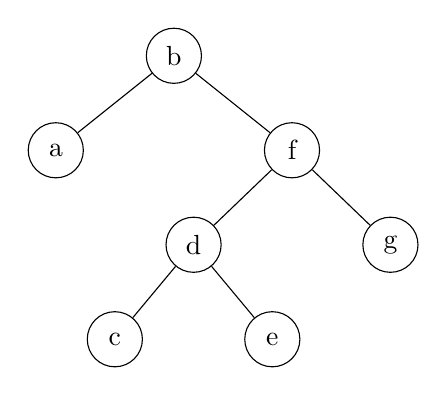
\begin{tikzpicture}[
    node style/.style={circle, draw, fill=white, minimum size=0.7cm, inner sep=0pt},
    level 1/.style={sibling distance=3cm, level distance=1.2cm},
    level 2/.style={sibling distance=2.5cm, level distance=1.2cm},
    level 3/.style={sibling distance=2cm, level distance=1.2cm}
]
\node[node style] (b) {b}
    child { node[node style] (a) {a} }
    child { node[node style] (f) {f}
        child { node[node style] (d) {d}
            child { node[node style] (c) {c} }
            child { node[node style] (e) {e} }
        }
        child { node[node style] (g) {g} }
    };
\end{tikzpicture}
\end{center}
节点c刚被访问完毕时栈中的元素从栈顶到栈底为: \\
A. d, c, f \\
B. d, f \\
C. f, g, d, e \\
D. d
\end{graybox}

\begin{solution}
正确答案是 B。

\textbf{详细分析:}
我们使用标准的迭代中序遍历算法,该算法使用一个栈。算法步骤如下:
\begin{enumerate}
    \item 初始化一个空栈 S。
    \item 初始化当前节点 \texttt{current} 为根节点。
    \item 当 \texttt{current} 不为 null 或者栈 S 不为空时,循环执行:
    \begin{enumerate}
        \item 当 \texttt{current} 不为 null 时:
        \begin{enumerate}
            \item 将 \texttt{current} 压入栈 S。
            \item 将 \texttt{current} 更新为其左孩子 (\texttt{current = current.left})。
        \end{enumerate}
        \item (此时 \texttt{current} 为 null,表示已到达最左侧)
        \begin{enumerate}
            \item 从栈 S 中弹出一个节点,设为 \texttt{popped\_node}。
            \item 访问 \texttt{popped\_node}。
            \item 将 \texttt{current} 更新为 \texttt{popped\_node} 的右孩子 (\texttt{current = popped\_node.right})。
        \end{enumerate}
    \end{enumerate}
\end{enumerate}

树的结构为:
\begin{verbatim}
      b
    /    \
   a      f
         / \
        d   g
       / \
      c   e
\end{verbatim}
栈的表示中,列表的右侧为栈顶。

\textbf{遍历过程追踪:}
\begin{enumerate}
    \item 初始:S = \texttt{[]}, \texttt{current} = \texttt{b}, 已访问 = \texttt{[]}
    \item \texttt{current} (\texttt{b}) 非空:
        \begin{itemize}
            \item \texttt{S.push(b)} $\rightarrow$ S = \texttt{[b]}
            \item \texttt{current = b.left} $\rightarrow$ \texttt{current} = \texttt{a}
        \end{itemize}
    \item \texttt{current} (\texttt{a}) 非空:
        \begin{itemize}
            \item \texttt{S.push(a)} $\rightarrow$ S = \texttt{[b, a]}
            \item \texttt{current = a.left} $\rightarrow$ \texttt{current} = null
        \end{itemize}
    \item \texttt{current} (null) 为空:
        \begin{itemize}
            \item \texttt{popped\_node = S.pop()} (弹出 \texttt{a}) $\rightarrow$ S = \texttt{[b]}
            \item 访问 \texttt{a}. 已访问 = \texttt{[a]}.
            \item \texttt{current = a.right} $\rightarrow$ \texttt{current} = null
        \end{itemize}
    \item \texttt{current} (null) 为空, 栈非空:
        \begin{itemize}
            \item \texttt{popped\_node = S.pop()} (弹出 \texttt{b}) $\rightarrow$ S = \texttt{[]}
            \item 访问 \texttt{b}. 已访问 = \texttt{[a, b]}.
            \item \texttt{current = b.right} $\rightarrow$ \texttt{current} = \texttt{f}
        \end{itemize}
    \item \texttt{current} (\texttt{f}) 非空:
        \begin{itemize}
            \item \texttt{S.push(f)} $\rightarrow$ S = \texttt{[f]}
            \item \texttt{current = f.left} $\rightarrow$ \texttt{current} = \texttt{d}
        \end{itemize}
    \item \texttt{current} (\texttt{d}) 非空:
        \begin{itemize}
            \item \texttt{S.push(d)} $\rightarrow$ S = \texttt{[f, d]}
            \item \texttt{current = d.left} $\rightarrow$ \texttt{current} = \texttt{c}
        \end{itemize}
    \item \texttt{current} (\texttt{c}) 非空:
        \begin{itemize}
            \item \texttt{S.push(c)} $\rightarrow$ S = \texttt{[f, d, c]}
            \item \texttt{current = c.left} $\rightarrow$ \texttt{current} = null
        \end{itemize}
    \item \texttt{current} (null) 为空:
        \begin{itemize}
            \item \texttt{popped\_node = S.pop()} (弹出 \texttt{c}) $\rightarrow$ S = \texttt{[f, d]}
            \item 访问 \texttt{c}. 已访问 = \texttt{[a, b, c]}.
            \item \textbf{此时是“节点c刚被访问完毕时”。}
            \item 栈 S 的内容为 \texttt{[f, d]}。
            \item 从栈顶到栈底的元素依次为: \texttt{d, f}。
            \item \texttt{current = c.right} $\rightarrow$ \texttt{current} = null
        \end{itemize}
\end{enumerate}
根据追踪,在节点 \texttt{c} 刚被访问完毕时,栈中的元素从栈顶到栈底依次为 \texttt{d, f}。
因此,选项 B 正确。
\end{solution}



\section*{88}
\begin{graybox}
对以下二叉树进行层次遍历:
\begin{lstlisting}
        a
      /
     b
    /   \
  c     d
        /.  \
      e     f
       \
        g
\end{lstlisting}
节点F正欲出队时队列中的元素从队头到队尾
为: \\
A. F \\
B. F,G \\
C. E,F \\
D. E,F,G
\end{graybox}

\begin{solution}
正确答案是 B。

\textbf{详细分析:}

首先,我们根据ASCII图确定二叉树的结构:
\begin{itemize}
    \item 节点 \texttt{a} 的左孩子是 \texttt{b},没有右孩子。
    \item 节点 \texttt{b} 的左孩子是 \texttt{c},右孩子是 \texttt{d}。
    \item 节点 \texttt{c} 没有孩子。
    \item 节点 \texttt{d} 的左孩子是 \texttt{e},右孩子是 \texttt{f} (根据 \texttt{d / . \\ e   f})。
    \item 节点 \texttt{e} 没有左孩子,右孩子是 \texttt{g} (根据 \texttt{e \\ \\ g})。
    \item 节点 \texttt{f} 没有孩子。
    \item 节点 \texttt{g} 没有孩子。
\end{itemize}
可视化树结构:
\begin{verbatim}
        a
       /
      b
     / \
    c   d
       / \
      e   f
       \
        g
\end{verbatim}

层次遍历使用队列 (Q) 来实现。我们将队列的左侧视为队头,右侧视为队尾。
\begin{enumerate}
    \item 初始:Q = \texttt{[]}, 已访问 = \texttt{[]}
    \item 将根节点 \texttt{a} 入队。Q = \texttt{[a]}
    \item \texttt{a} 出队。访问 \texttt{a}。已访问 = \texttt{[a]}。
          \texttt{a} 的左孩子 \texttt{b} 入队。Q = \texttt{[b]}。
          (\texttt{a} 没有右孩子)
    \item \texttt{b} 出队。访问 \texttt{b}。已访问 = \texttt{[a, b]}。
          \texttt{b} 的左孩子 \texttt{c} 入队。Q = \texttt{[c]}。
          \texttt{b} 的右孩子 \texttt{d} 入队。Q = \texttt{[c, d]}。
    \item \texttt{c} 出队。访问 \texttt{c}。已访问 = \texttt{[a, b, c]}。
          (\texttt{c} 没有孩子)
          Q = \texttt{[d]}。
    \item \texttt{d} 出队。访问 \texttt{d}。已访问 = \texttt{[a, b, c, d]}。
          \texttt{d} 的左孩子 \texttt{e} 入队。Q = \texttt{[e]}。
          \texttt{d} 的右孩子 \texttt{f} 入队。Q = \texttt{[e, f]}。
    \item \texttt{e} 出队。访问 \texttt{e}。已访问 = \texttt{[a, b, c, d, e]}。
          (\texttt{e} 没有左孩子)
          \texttt{e} 的右孩子 \texttt{g} 入队。Q = \texttt{[f, g]}。
    \item \textbf{此时,节点 \texttt{f} 位于队头,正欲出队。}
          队列 Q 中的元素从队头到队尾依次为: \texttt{f, g}。
\end{enumerate}
(遍历继续)
\begin{enumerate}
    \item[8.] \texttt{f} 出队。访问 \texttt{f}。已访问 = \texttt{[a, b, c, d, e, f]}。
          (\texttt{f} 没有孩子)
          Q = \texttt{[g]}。
    \item[9.] \texttt{g} 出队。访问 \texttt{g}。已访问 = \texttt{[a, b, c, d, e, f, g]}。
          (\texttt{g} 没有孩子)
          Q = \texttt{[]}。
\end{enumerate}
根据追踪,在节点 \texttt{f} 正欲出队时,队列中的元素从队头到队尾为 \texttt{f, g}。
因此,选项 B 正确。
\end{solution}


\section*{89}
\begin{graybox}
后序遍历序列中最后一个节点是: \\
A. 根节点 \\
B. 最左边的节点 \\
C. 最右边的节点 \\
D. 深度最大的节点
\end{graybox}

\begin{solution}
正确答案是 A。

\textbf{详细分析:}

二叉树的后序遍历遵循“左-右-根”的顺序。这意味着:
\begin{enumerate}
    \item 对当前节点的左子树进行后序遍历。
    \item 对当前节点的右子树进行后序遍历。
    \item 访问当前节点(根节点)。
\end{enumerate}

根据这个递归定义,当对整棵树进行后序遍历时:
\begin{itemize}
    \item 首先,整个左子树会被完整地以后序遍历的方式访问。
    \item 其次,整个右子树会被完整地以后序遍历的方式访问。
    \item 最后,树的根节点本身才会被访问。
\end{itemize}
因此,在后序遍历序列中,树的根节点总是最后一个被访问的节点。

分析选项:
\begin{itemize}
    \item \textbf{A. 根节点:} 这是正确的。根据“左-右-根”的顺序,根节点在其所有子孙节点都被访问之后才被访问。
    \item \textbf{B. 最左边的节点:} 最左边的节点通常是中序遍历中第一个被访问的节点。在后序遍历中,它会在其右兄弟(如果存在)和其父节点之前被访问,但不是最后一个。
    \item \textbf{C. 最右边的节点:} 最右边的节点在其左兄弟(如果存在)和其父节点之前被访问(如果它是叶子节点),但也不是最后一个,除非它本身就是根节点且没有左子树。
    \item \textbf{D. 深度最大的节点:} 深度最大的节点(通常是叶子节点)会在其父节点之前被访问,但根节点是最后一个。例如,在一个简单的链状树 A $\rightarrow$ B $\rightarrow$ C (A是根, B是A的左孩子, C是B的左孩子),后序遍历是 C, B, A。C是深度最大的,但A(根节点)是最后一个。
\end{itemize}

因此,后序遍历序列中最后一个节点是树的根节点。
\end{solution}


\section*{90}
\begin{graybox}
下列关于树的命题中错误的是: \\
A. 顶点数为n的树的边数为n-1。 \\
B. 树中任意两顶点之间存在唯一路径。 \\
C. 在树中添加任一条边都会破坏树的结构。 \\
D. 在树中删除任一条边得到的还是树
\end{graybox}

\begin{solution}
正确答案是 D。

\textbf{详细分析:}

\begin{itemize}
    \item \textbf{A. 顶点数为n的树的边数为n-1。}
        这是树的一个基本性质。一个无向图是树的充要条件之一是:图是连通的,并且有 $n$ 个顶点和 $n-1$ 条边。或者,图是无环的,并且有 $n$ 个顶点和 $n-1$ 条边。
        \textbf{这个命题是正确的。}

    \item \textbf{B. 树中任意两顶点之间存在唯一路径。}
        这也是树的一个基本定义或性质。如果任意两顶点之间存在多于一条路径,那么这些路径必然会形成一个环,而树是无环图。如果某些顶点之间不存在路径,则图不连通,也不是树。
        \textbf{这个命题是正确的。}

    \item \textbf{C. 在树中添加任一条边都会破坏树的结构。}
        “破坏树的结构”意味着结果不再是树。如果在树中任意两个不相邻的顶点之间添加一条新的边,由于这两个顶点之间已经存在一条唯一的路径,新添加的边会与这条路径形成一个环。树的定义是无环连通图,所以添加边后形成的图将不再是树(因为它包含了环)。
        \textbf{这个命题是正确的。}

    \item \textbf{D. 在树中删除任一条边得到的还是树。}
        树是连通的。如果从树中删除任意一条边,这条边必然是一个桥(割边),即删除它会导致图不再连通(除非原树只有一个顶点,没有边,或者只有两个顶点一条边,删除后剩孤立点)。如果图不再连通,它就不再是一棵树,而变成了一个森林(由两个或多个树组成的图)。
        例如,一个有3个顶点A, B, C和两条边 (A,B), (B,C) 的树。如果删除边 (A,B),则A变成孤立点,图不再连通,不再是树。
        \textbf{这个命题是错误的。}
\end{itemize}

因此,错误的命题是 D。
\end{solution}


\section*{91}
\begin{graybox}
从n个节点的二叉树的叶节点u逐个节点地上溯
到根节点的过程中,以下说法中错误的是: \\
A. 经过的节点都是u的祖先。 \\
B. 最坏时间复杂度为O(n) \\
C. 经过的路径是唯一确定的 \\
D. 每上溯一层,当前节点的深度减小1,而高度增
加1。
\end{graybox}

\begin{solution}
正确答案是 D。

\textbf{详细分析:}

\begin{itemize}
    \item \textbf{A. 经过的节点都是u的祖先。}
        当从叶节点u上溯到根节点时,经过的每一个中间节点(除了u本身)都是u的父节点、祖父节点等,直到根节点。这些节点按定义都是u的祖先。
        \textbf{这个命题是正确的。}

    \item \textbf{B. 最坏时间复杂度为O(n)。}
        上溯的路径长度等于叶节点u的深度。在一棵有n个节点的二叉树中,最坏情况下(例如,一个退化为链表的树),一个叶节点的深度可以是 $n-1$。因此,上溯过程访问的节点数最多为 $n$(包括叶节点和根节点)。所以,最坏时间复杂度是 $O(n)$。
        \textbf{这个命题是正确的。}

    \item \textbf{C. 经过的路径是唯一确定的。}
        在树结构中,每个节点(除了根节点)有且仅有一个父节点。因此,从任何节点u向上到根节点的路径是唯一的,因为每一步都只能走向唯一的父节点。
        \textbf{这个命题是正确的。}

    \item \textbf{D. 每上溯一层,当前节点的深度减小1,而高度增加1。}
        \begin{itemize}
            \item \textbf{深度:} 节点的深度是从根节点到该节点的路径长度。根节点的深度为0。当从一个节点 $v$ 上溯到其父节点 $p$ 时,与根节点的距离减少了1。所以,当前节点的深度确实减小1。
            \item \textbf{高度:} 节点的高度是从该节点到其子树中某个叶子节点的最长路径的长度。叶子节点的高度为0。
            设当前节点为 $v$,其父节点为 $p$。
            $height(p) = 1 + \max(\text{height of } p\text{'s children})$ (如果 $p$ 不是叶子)。
            当从子节点 $v$ 上溯到父节点 $p$ 时,我们比较 $height(v)$ 和 $height(p)$。
            $height(p)$ 不一定等于 $height(v) + 1$。
            例如,考虑树:
            \begin{verbatim}
                  A (h=2)
                 / \
                B   C (h=1)
               (h=0) \
                      D (h=0)
            \end{verbatim}
            如果从叶节点 B (深度2, 高度0) 上溯到其父节点 A (深度1, 高度2)。
            深度从2减小到1 (减小1)。
            高度从0增加到2 (增加2,而不是1)。
            这是因为 A 的高度是由其另一个孩子 C 决定的 ($height(A) = 1 + height(C) = 1+1=2$)。
            因此,“高度增加1”这个部分是错误的。
        \end{itemize}
        由于“高度增加1”不总是成立,所以整个命题D是错误的。
        \textbf{这个命题是错误的。}
\end{itemize}

因此,错误的说法是 D。
\end{solution}


\section*{92}
\begin{graybox}
对二叉树进行中序遍历,节点v在中序遍
历下的后继为(假设v的后继存在): \\
A. 其右子树中第一个被访问的节点 \\
B. 其左子树中第一个被访问的节点 \\
C. 其右子树中第一个被访问的节点或v的某个
祖先 \\
D. 其右子树中第一个被访问的节点或其左子
树中的某个节点
\end{graybox}

\begin{solution}
正确答案是 C。

\textbf{详细分析:}

中序遍历的顺序是“左-根-右”。节点 $v$ 的中序后继是指在中序遍历序列中紧跟在 $v$ 后面的那个节点。

有两种主要情况:

\textbf{情况 1: 节点 $v$ 有右子树。}
如果节点 $v$ 有一个右子树,那么根据“左-根-右”的顺序,在访问完 $v$(根)之后,接下来会遍历 $v$ 的右子树。在 $v$ 的右子树中,第一个被访问的节点将是该右子树中“最左边”的节点。这个节点就是 $v$ 的中序后继。
所以,如果 $v$ 有右子树,其后继是“其右子树中第一个被访问的节点”(即右子树的最左节点)。

\textbf{情况 2: 节点 $v$ 没有右子树。}
如果节点 $v$ 没有右子树,那么 $v$ 的中序后继是 $v$ 的某个祖先。具体来说,它是 $v$ 的“最低的祖先节点 $p$,使得 $v$ 位于 $p$ 的左子树中”。
我们可以从 $v$ 开始向上回溯其父节点:
\begin{itemize}
    \item 如果 $v$ 是其父节点 $p$ 的左孩子,那么父节点 $p$ 就是 $v$ 的中序后继。
    \item 如果 $v$ 是其父节点 $p$ 的右孩子,那么 $p$ 及其左子树都已经访问过了(在 $v$ 之前)。我们需要继续向上找,直到找到一个节点 $a$,使得当前路径是从 $a$ 的左分支下来的。这个节点 $a$ 就是 $v$ 的后继。
\end{itemize}
在这种情况下,后继是 $v$ 的一个祖先。

综合这两种情况:
\begin{itemize}
    \item 如果 $v$ 有右子树,后继在右子树中。
    \item 如果 $v$ 没有右子树,后继是 $v$ 的某个祖先。
\end{itemize}

分析选项:
\begin{itemize}
    \item \textbf{A. 其右子树中第一个被访问的节点:} 这只覆盖了情况1。如果 $v$ 没有右子树,这个说法就不适用。
    \item \textbf{B. 其左子树中第一个被访问的节点:} 左子树中的节点在中序遍历中总是在 $v$ 之前被访问,所以不可能是后继。
    \item \textbf{C. 其右子树中第一个被访问的节点或v的某个祖先:} 这个选项正确地包含了上述两种情况。如果 $v$ 有右子树,则后继是右子树中的第一个被访问的节点;如果 $v$ 没有右子树,则后继是 $v$ 的某个祖先。
    \item \textbf{D. 其右子树中第一个被访问的节点或其左子树中的某个节点:} 左子树中的节点不可能是后继。
\end{itemize}

因此,选项 C 是最全面和正确的描述。
\end{solution}


\section*{93}
\begin{graybox}
与先序、中序遍历类似,以左子->右子->根
节点的顺序来访问二叉树称为后序遍历。后序遍历
中第一个被访问的节点是: \\
A. 左侧链中最深的节点 \\
B. 根节点 \\
C. 右侧链中最深的节点 \\
D. 以上皆不是
\end{graybox}

\begin{solution}
正确答案是 D。

\textbf{详细分析:}

后序遍历的顺序是“左子树 -> 右子树 -> 根节点”。
要找到第一个被访问的节点,我们需要遵循这个规则,深入到树的某个部分,直到找到一个节点,其左子树和右子树都(被认为是)已经处理完毕(对于第一个节点,这意味着它的左子树和右子树都是空的,即它是一个叶子节点),然后这个节点本身被访问。

具体来说,第一个被访问的节点是这样找到的:
\begin{enumerate}
    \item 从当前节点开始,尝试访问其左子树。不断深入左子节点。
    \item 如果到达一个没有左子节点的节点N,则尝试访问N的右子树。
    \item 如果N也没有右子节点(即N是一个叶子节点),那么N就是第一个被访问的节点。
    \item 如果N有右子节点M,则对M的子树重复此过程(先深入M的左子树,再深入M的右子树)。
\end{enumerate}
所以,第一个被访问的节点总是树中的一个叶子节点。它是通过优先向左,然后在无法向左时转向右,并再次优先向左,直到到达一个叶子节点。这个叶子节点可以被认为是树的“最左边的可用叶子节点”。

现在我们分析选项:
\begin{itemize}
    \item \textbf{A. 左侧链中最深的节点:}
        “左侧链”通常指从根节点开始,只通过左孩子指针连接的节点序列。该链中最深的节点是此序列的最后一个节点。
        考虑以下例子:
        \begin{verbatim}
              A
             /
            B  <-- B是A的左侧链中最深的节点
             \
              C
             /
            D  <-- D是后序遍历中第一个被访问的节点
        \end{verbatim}
        后序遍历顺序是 D, C, B, A。第一个被访问的节点是D。
        A的左侧链是 A $\rightarrow$ B。此链中最深的节点是B。
        由于 D $\neq$ B,所以这个命题不总是成立。

    \item \textbf{B. 根节点:}
        在后序遍历中,根节点是在其所有子孙节点都被访问之后,最后一个被访问的节点。所以这个命题是错误的。

    \item \textbf{C. 右侧链中最深的节点:}
        这不符合后序遍历首先探索左子树的特性。所以这个命题是错误的。

    \item \textbf{D. 以上皆不是:}
        由于选项A在某些情况下不成立(如上例所示),且B和C是明显错误的,因此这个选项是正确的。
\end{itemize}

第一个被访问的节点是树的“最左下的叶子节点”(leftmost leaf after exhausting leftward paths, then rightward paths that lead to further leftward paths)。这个描述不直接对应选项A、B或C中的任何一个的严格定义。
\end{solution}

\section*{94}
\begin{graybox}
对二叉树进行先序遍历,u和v是左侧链
上两个节点,且u是v的祖先,x、y分别是u和
v的右子,试问这四个节点被访问的顺序是: \\
A. y,v,x,u \\
B. x,y,v,u \\
C. u,v,y,x \\
D. unconfirmed无法确定
\end{graybox}

\begin{solution}
正确答案是 C。

\textbf{详细分析:}

先序遍历的顺序是:根节点 $\rightarrow$ 左子树 $\rightarrow$ 右子树。

根据题目描述:
\begin{itemize}
    \item \texttt{u} 和 \texttt{v} 是左侧链上的两个节点。
    \item \texttt{u} 是 \texttt{v} 的祖先。这意味着在从根节点到 \texttt{v} 的路径上,\texttt{u} 出现在 \texttt{v} 之前,并且 \texttt{v} 位于 \texttt{u} 的左子树中(因为它们都在左侧链上,且u是v的祖先)。
    \item \texttt{x} 是 \texttt{u} 的右孩子。
    \item \texttt{y} 是 \texttt{v} 的右孩子。
\end{itemize}

我们可以描绘出这些节点之间关系的一个大致结构:
\begin{verbatim}
      ...
      |
      u
     / \
    L_u x   (L_u 是 u 的左孩子,v 在 L_u 的子树中或 L_u 就是 v)
   /
  ...
 /
v
 \
  y     (v 的左孩子,如果存在,会是左侧链上更深的节点)
\end{verbatim}

现在我们追踪先序遍历的访问顺序:
\begin{enumerate}
    \item \textbf{访问 \texttt{u}:}
    当遍历到达节点 \texttt{u} 时,\texttt{u} 首先被访问(作为其子树的根)。
    访问序列目前:\texttt{u}

    \item \textbf{遍历 \texttt{u} 的左子树:}
    接下来,遍历 \texttt{u} 的左子树。由于 \texttt{v} 在 \texttt{u} 的左子树中(并且在左侧链上),遍历最终会到达 \texttt{v}。
    \begin{itemize}
        \item 当遍历到达节点 \texttt{v} 时,\texttt{v} 被访问(作为其子树的根)。
        访问序列目前:\texttt{u, v}
        \item 接下来,遍历 \texttt{v} 的左子树。这部分不包含 \texttt{x} 或 \texttt{y}。
        \item 在 \texttt{v} 的左子树遍历完毕后,遍历 \texttt{v} 的右子树。节点 \texttt{y} 是 \texttt{v} 的右孩子,所以 \texttt{y} 会被访问。
        访问序列目前:\texttt{u, v, y}
        \item 之后遍历 \texttt{y} 的子树。
    \end{itemize}
    在 \texttt{u} 的整个左子树(包含 \texttt{v} 和 \texttt{y} 及其子树)被遍历完毕后,控制返回。

    \item \textbf{遍历 \texttt{u} 的右子树:}
    在 \texttt{u} 本身及其整个左子树都被访问之后,接下来遍历 \texttt{u} 的右子树。节点 \texttt{x} 是 \texttt{u} 的右孩子,所以 \texttt{x} 会被访问。
    访问序列目前:\texttt{u, v, y, x}
    \item 之后遍历 \texttt{x} 的子树。
\end{enumerate}

因此,这四个节点 \texttt{u, v, x, y} 被访问的顺序是 \texttt{u, v, y, x}。

对照选项:
A. y,v,x,u - 错误
B. x,y,v,u - 错误
C. u,v,y,x - 正确
D. unconfirmed无法确定 - 错误,可以确定。

\end{solution}



\section*{95}
\begin{graybox}
关于二叉树遍历序列之间关系的说法错误的是: \\
A. 已知先序遍历序列和中序遍历序列可以确定后序遍历序列 \\
B. 已知中序遍历序列和后序遍历序列可以确定先序遍历序列 \\
C. 已知中序遍历序列和后序遍历序列可以确定层次遍历序列 \\
D. 已知先序遍历序列和后序遍历序列可以确定中序遍历序列
\end{graybox}

\begin{solution}
正确答案是 D。

\textbf{详细分析:}

\begin{itemize}
    \item \textbf{A. 已知先序遍历序列和中序遍历序列可以确定后序遍历序列。}
        这是正确的。先序遍历的第一个元素是树的根。在中序遍历中找到这个根元素,可以将中序序列分为左子树和右子树。然后可以递归地对左子树和右子树的先序和中序子序列进行同样的操作,从而唯一地重建整个二叉树。一旦树被唯一确定,其后序遍历序列也随之唯一确定。

    \item \textbf{B. 已知中序遍历序列和后序遍历序列可以确定先序遍历序列。}
        这是正确的。后序遍历的最后一个元素是树的根。在中序遍历中找到这个根元素,可以将中序序列分为左子树和右子树。然后可以递归地对左子树和右子树的后序和中序子序列进行同样的操作,从而唯一地重建整个二叉树。一旦树被唯一确定,其先序遍历序列也随之唯一确定。

    \item \textbf{C. 已知中序遍历序列和后序遍历序列可以确定层次遍历序列。}
        这是正确的。如B所述,已知中序遍历和后序遍历可以唯一确定二叉树的结构。一旦二叉树的结构被确定,就可以通过标准的层次遍历算法(通常使用队列)得到其唯一的层次遍历序列。

    \item \textbf{D. 已知先序遍历序列和后序遍历序列可以确定中序遍历序列。}
        \textbf{这是错误的。} 仅凭先序遍历序列和后序遍历序列,通常不足以唯一确定一棵二叉树(中序遍历序列)。
        例如,考虑以下两种不同的二叉树:
        \textbf{树1:}
        \begin{verbatim}
            A
           /
          B
        \end{verbatim}
        先序: A, B
        后序: B, A
        中序: B, A

        \textbf{树2:}
        \begin{verbatim}
            A
             \
              B
        \end{verbatim}
        先序: A, B
        后序: B, A
        中序: A, B

        树1和树2有相同的先序遍历序列 (A, B) 和相同的后序遍历序列 (B, A),但它们的中序遍历序列不同。因此,仅凭先序和后序序列无法唯一确定中序序列或树的结构。
        (注意:如果二叉树是满二叉树或完全二叉树,或者更一般地,如果树中没有度为1的节点,则先序和后序可以唯一确定树。但题目中说的是一般的“二叉树”。)
\end{itemize}

因此,错误的说法是 D。
\end{solution}




\section*{96}
\begin{graybox}
借助队列对二叉树进行层次遍历时,任意
时刻队列中的节点满足: \\
A. 均位于从根节点到当前节点的路径上 \\
B. 均是当前节点的后代 \\
C. 高度相差不超过1 \\
D. 深度相差不超过1
\end{graybox}

\begin{solution}
正确答案是 D。

\textbf{详细分析:}

层次遍历(Level-order Traversal)使用队列来存储待访问的节点。其过程是:
\begin{enumerate}
    \item 将根节点入队。
    \item 当队列不为空时,执行以下操作:
    \begin{enumerate}
        \item 将队头节点出队,并访问该节点(称之为“当前处理的节点”)。
        \item 如果当前处理的节点的左孩子存在,则将其左孩子入队。
        \item 如果当前处理的节点的右孩子存在,则将其右孩子入队。
    \end{enumerate}
\end{enumerate}

我们来分析各个选项:

\begin{itemize}
    \item \textbf{A. 均位于从根节点到当前节点的路径上:}
        “当前节点”通常指刚刚出队并被访问的节点。队列中的其他节点是当前节点尚未处理的兄弟节点(同一层)或者是下一层的节点(当前节点或其兄弟节点的孩子)。这些节点不一定位于从根到当前已访问节点的路径上。例如,如果队列中有A的两个孩子B和C,当B出队被访问时,C仍在队列中,但C不在根到B的路径上。所以A是错误的。

    \item \textbf{B. 均是当前节点的后代:}
        同样,“当前节点”指刚出队的节点。队列中的节点可能是当前节点的兄弟节点(同一层)或下一层的节点。它们不全是当前已访问节点的后代。例如,当根节点A出队后,其孩子B、C入队。此时队列中是B和C,它们不是A的后代(它们是A的孩子)。如果B出队,队列中是C,C不是B的后代。所以B是错误的。

    \item \textbf{C. 高度相差不超过1:}
        节点的高度是从该节点到其子树中某个叶子节点的最长路径长度。
        考虑以下树:
        \begin{verbatim}
              A (h=3)
             / \
            B(h=2) G(h=0)
           /
          C(h=1)
         /
        D(h=0)
        \end{verbatim}
        当A出队后,B和G入队。队列为 [B, G]。
        高度(B) = 2, 高度(G) = 0。高度差为 $2 - 0 = 2$,这超过了1。
        所以C是错误的。

    \item \textbf{D. 深度相差不超过1:}
        节点的深度是从根节点到该节点的路径长度。根节点的深度为0。
        在层次遍历中,我们逐层处理节点。
        \begin{itemize}
            \item 开始时,队列中只有根节点(深度0)。
            \item 当处理深度为 $k$ 的节点时,这些节点会从队列中出队。它们的孩子(深度为 $k+1$)会被入队。
            \item 因此,在任意时刻,队列中的节点要么都属于同一深度 $k$,要么属于相邻的两个深度 $k$ 和 $k+1$。
                \begin{itemize}
                    \item 如果队列中所有节点都来自同一深度 $k$,则它们之间的深度差为0。
                    \item 如果队列中包含深度为 $k$ 的节点(尚未处理完)和深度为 $k+1$ 的节点(已处理的深度 $k$ 节点的子节点),则任意两个节点之间的深度差最大为 $(k+1) - k = 1$。
                \end{itemize}
        \end{itemize}
        因此,任意时刻队列中的节点深度相差不超过1。
        \textbf{这个命题是正确的。}
\end{itemize}
\end{solution}














\end{document}

% VScode 常用快捷键:

% Ctrl + R:                 打开最近的文件夹
% F2:                       变量重命名
% Ctrl + Enter:             行中换行
% Alt + up/down:            上下移行
% 鼠标中键 + 移动:           快速多光标
% Shift + Alt + up/down:    上下复制
% Ctrl + left/right:        左右跳单词
% Ctrl + Backspace/Delete:  左右删单词    
% Shift + Delete:           删除此行
% Ctrl + J:                 打开 VScode 下栏(输出栏)
% Ctrl + B:                 打开 VScode 左栏(目录栏)
% Ctrl + `:                 打开 VScode 终端栏
% Ctrl + 0:                 定位文件
% Ctrl + Tab:               切换已打开的文件(切标签)
% Ctrl + Shift + P:         打开全局命令(设置)

% Latex 常用快捷键

% Ctrl + Alt + J:           由代码定位到PDF
% 


% Git提交规范:
% update: Linear Algebra 2 notes
% add: Linear Algebra 2 notes
% import: Linear Algebra 2 notes
% delete: Linear Algebra 2 notes
